%%% LaTeX template
%%% Dae Houlihan

%%%%%%%%%%%%%%%%%%%%%%%
%%% Document setup
%%%%%%%%%%%%%%%%%%%%%%%

\documentclass[12pt,letterpaper]{article}

\usepackage[english]{babel}

\usepackage{cmap} % provides character map tables, which make PDF files generated by pdfLATEX both searchable and copy-able in acrobat reader and other compliant PDF viewers

%%% for pdflatex %%% see https://tex.stackexchange.com/questions/44694/fontenc-vs-inputenc
\usepackage[T1]{fontenc} % use 8-bit T1 fonts; oriented to output, that is, what fonts to use for printing characters
\usepackage[utf8]{inputenc} % allow utf-8 input; allows the user to input accented characters directly from the keyboard
%%% The two packages are not connected, though it is best to call fontenc first and then inputenc %%%

%%% If you use \usepackage[T1]{fontenc} with Computer Modern, it uses bitmap fonts which end up pixelated. Latin Modern doesn't suffer from this problem %%%
\usepackage{lmodern}

%%% Set page size and margins %%%
\usepackage[letterpaper,top=2cm,bottom=2cm,left=3cm,right=3cm,marginparwidth=1.75cm]{geometry}

\usepackage[font={small}]{caption} % format captions font

%%%%%%%%%%%%%%%%%%%%%%%
%%% BibLaTeX with biber backend
%%%%%%%%%%%%%%%%%%%%%%%

\usepackage[
    backend=biber,
    style=apa,
    natbib=true,
    url=false, 
    doi=true,
    eprint=false,
%    uniquename=false,
%    giveninits=false,
%    uniquelist=false,
]{biblatex}
\addbibresource{bibliography.bib}
%%% have in-parentheses citation notes separated by ; rather than , %%%
%\setcitestyle{citesep={;}}
\renewcommand*{\postnotedelim}{\addsemicolon\space}


%%%%%%%%%%%%%%%%%%%%%%%
%%% Packages
%%%%%%%%%%%%%%%%%%%%%%%

\usepackage{url} % simple URL typesetting
\usepackage{booktabs} % professional-quality tables
\usepackage{graphicx}
\usepackage{mathtools}
\usepackage{amsfonts} % blackboard math symbols
\usepackage{amsmath}
\usepackage{amssymb}
\usepackage{csquotes}
\usepackage{nicefrac} % compact symbols for 1/2, etc.
\usepackage{pifont} % special characters like dings
\usepackage{bm,microtype} % italic bold math % microtypography % for some reason microtype turns off Texifier live
\usepackage{xspace} % for variable formatting

\usepackage{placeins} % control float placement with \FloatBarrier
\usepackage{comment} % \begin{comment}\end{comment} environment

\usepackage{authblk} % for author affiliations

\usepackage[raggedright]{titlesec} %%% don't hyphenate titles

%\usepackage{lgrind} % prepares various programming language source code for pretty-printing


%%%%%%%%%%%%%%%%%%%%%%%
%%% Variable formatting
%%%%%%%%%%%%%%%%%%%%%%%

%%%%%%%%%
%%% Hyphenation
%%%%%%%%%

\hyphenation{Golden-Balls}

%%%%%%%%%
%%% Acronyms
%%%%%%%%%

\newcommand*{\DefaultAcronymStyle}[1]{#1}
\newcommand*{\Acronym}[2][\DefaultAcronymStyle]{\expandafter\def\csname #2\endcsname{#1{#2}\xspace}}

\Acronym{ToM}
\Acronym[\textsc]{BToM}

%%%%%%%%%
%%% Greek variants
%%%%%%%%%

\newcommand*{\swap}[2]{\let\temp#1 \let#1#2 \let#2\temp \let\temp\relax}
\swap{\epsilon}{\varepsilon}
%\swap{\theta}{\vartheta}
\swap{\phi}{\varphi}

%%%%%%%%%
%%% Text commands
%%% (N.B \newcommand can contain \par, \newcommand* cannot)
%%%%%%%%%

\xspaceaddexceptions{]\}} %%% prevents extra spaces when command is closed with ] or }

\newcommand*{\ie}{i.e.\xspace}
\newcommand*{\eg}{e.g.\xspace}
\newcommand*{\Ie}{I.e.\xspace}
\newcommand*{\Eg}{E.g.\xspace}

\newcommand*{\cmark}{\ding{51}}%
\newcommand*{\xmark}{\ding{55}}%

\newcommand*{\somemarkup}{\texttt{SomeMarkup}\xspace}
\newcommand*{\somemodel}{\textsc{SomeModel}\xspace}

%%%%%%%%%
%%% Math commands
%%%%%%%%%

\DeclarePairedDelimiter{\abs}{\lvert}{\rvert}
\DeclarePairedDelimiter{\ceil}{\lceil}{\rceil}
\DeclarePairedDelimiter{\floor}{\lfloor}{\rfloor}
\DeclarePairedDelimiter{\paren}{\lparen}{\rparen}
\DeclarePairedDelimiter{\brak}{[}{]}
\DeclarePairedDelimiter{\setbrak}{\left\{}{\right\}}
\DeclarePairedDelimiter{\tuple}{\langle}{\rangle}
\def\pp#1{\paren*{#1}}

%\renewcommand*{\vec}[1]{{\bm{#1}}}
\let\vec\relax
\newcommand*{\vec}[1]{\bm{#1}}
\newcommand*{\mat}[1]{\bm{#1}}
\newcommand*{\mvec}[1]{\begin{pmatrix}#1\end{pmatrix}}

\DeclareMathOperator{\pr}{P}
\DeclareMathOperator{\giv}{\mid}
\DeclareMathOperator{\givmiddle}{\;\middle\vert\;}
\DeclareMathOperator{\param}{\,\!\mathbin{;}\,}

\DeclareMathOperator*{\E}{\mathbf{E}} %%% star takes subscripts below
\DeclareMathOperator{\Ee}{\mathbf{E}}

\DeclareMathOperator{\Like}{\mathcal{L}}
\DeclareMathOperator{\Lagr}{\ell}

\DeclareMathOperator{\Corr}{Corr}
\DeclareMathOperator{\Cov}{Cov}

\DeclareMathOperator*{\argmax}{argmax}


%%%%%%%%%%%%%%%%%%%%%%%
%%% Draft Markup
%%%%%%%%%%%%%%%%%%%%%%%

%%% DRAFT %%%
\usepackage[dvipsnames]{xcolor}
\definecolor{ccpink}{rgb}{0.858, 0.188, 0.478}
\definecolor{ccmulberry}{RGB}{168, 62, 158}
\definecolor{ccburentorange}{RGB}{193, 92, 0}
\definecolor{ccdgreen}{RGB}{0, 133, 19}
\definecolor{ccbrown}{RGB}{135, 32, 1}
\definecolor{lightgrey}{rgb}{0.95, 0.95, 0.95}
\newcommand{\wip}[1]{{\color{red}#1}}
\newcommand{\reword}[1]{{\color{ccbrown}#1}}
\newcommand{\hide}[1]{\ignorespaces}
\newcommand{\dae}[1]{{\color{ccmulberry}#1}}

%%% FINAL %%%
%\newcommand{\reword}[1]{#1}
%\newcommand{\hide}[1]{\ignorespaces}
%\newcommand{\dae}[1]{\ignorespaces}


%%%%%%%%%%%%%%%%%%%%%%%
%%% Regulate auto-hyphenation
%%%%%%%%%%%%%%%%%%%%%%%

\tolerance=9999 %% allows as much whitespace as possible.
%\emerencystretch=10pt %% allows some extra whitespace per line.
\hyphenpenalty=10000 %% disables hyphens completely.
\exhyphenpenalty=100 %% allows using hyphens which were already present.

%%%%%%%%%%%%%%%%%%%%%%%
%%% Internal links
%%%%%%%%%%%%%%%%%%%%%%%

\usepackage[colorlinks=true, allcolors=blue]{hyperref} % hyperlinks - best loaded at end of preamble
\usepackage{subfiles} % subfiles - best loaded last in the preamble

%%%%%%%%%%%%%%%%%%%%%%%
%%% Header
%%%%%%%%%%%%%%%%%%%%%%%

\title{LaTeX template, with BibLaTeX and biber backend}
\author[a,b]{Sean Dae Houlihan}
\affil[a]{Department of Psychological and Brain Sciences, Dartmouth College}
\affil[b]{Department of Brain and Cognitive Sciences, Massachusetts Institute of Technology}
\setcounter{Maxaffil}{0}
\renewcommand\Affilfont{\small}
\date{}

%%%%%%%%%%%%%%%%%%%%%%%%%%%%%%%%%%%%%%%%%%%%%%%%%%%%%%%%%%%%%%%%%%%%%
%%% DOCUMENT
%%%%%%%%%%%%%%%%%%%%%%%%%%%%%%%%%%%%%%%%%%%%%%%%%%%%%%%%%%%%%%%%%%%%%

\begin{document}
\maketitle

\begin{abstract}
\noindent 
This thesis develops a framework for computationally recapitulating human emotion understanding. I argue that expression cues and contextual information mutually constrain inference over an intuitive theory of mind. Emotion concepts reflect computations in the space of inferred appraisals, and inferred appraisals function as latent causal explanations that link expressions, actions, preferences, beliefs, costs, and world states across time. 
\end{abstract}


%%% relax \clearpage to prevent page breaks between subfiles, bibliography %%%

\begingroup
\let\clearpage\relax
\section{Introduction}

My research highlights the critical role of context, and of prediction, in emotion understanding. Contextual information shapes forward predictions of how others will interpret external events in relation to their mental contents (beliefs, desires, moral values, costs, etc.). These forward predictions in turn constrain ill-posed inverse inferences, allowing people to explain others' expressions and behavior \citep{saxe2017cop}. My results support the view that forward predictions guide inverse inferences about expressions. Contextual cues about what did happen, what could have happened, what someone wanted to happen, and what someone believed would happen, constrain the predictions generated by people's intuitive theory \citep{houlihan2018cogsci}. The contextual shaping of forward predictions in turn constrains the emotions attributed to expressions \citep{anzellotti2021emotion}, and the prior experiences inferred from from expressions \citep{houlihan2022emotionreasoning}. Knowing specifically what situations people were reacting to changes the emotions attributed to their expressions \citep{anzellotti2021emotion, houlihan2022thesis}. Knowing merely what events \emph{might} have transpired, but not what actually happened, also changes emotion attribution \citep{houlihan2022emotionreasoning, anzellotti2021emotion}.


\endgroup

\begingroup
\let\clearpage\relax
\printbibliography
\endgroup

\clearpage

\pagenumbering{arabic} %%% resets `page` counter to 1
\renewcommand*{\thepage}{S\arabic{page}}
\appendix

\setcounter{section}{0}
\makeatletter 
\renewcommand{\thesection}{S\@arabic\c@section}
\makeatother

\setcounter{figure}{0}
\makeatletter 
\renewcommand{\thefigure}{S\@arabic\c@figure}
\makeatother

\setcounter{table}{0}
\makeatletter 
\renewcommand{\thetable}{S\@arabic\c@table}
\makeatother

\section*{\centering {Supplementary Materials}} \label{sec:supplement}

\section{Some Examples}

Here are the supplementary materials. This is a dynamic input: $0.889~[0.880, 0.891]%$.

\subsection{Example Figure}

\begin{figure}[h!]
	\centering
	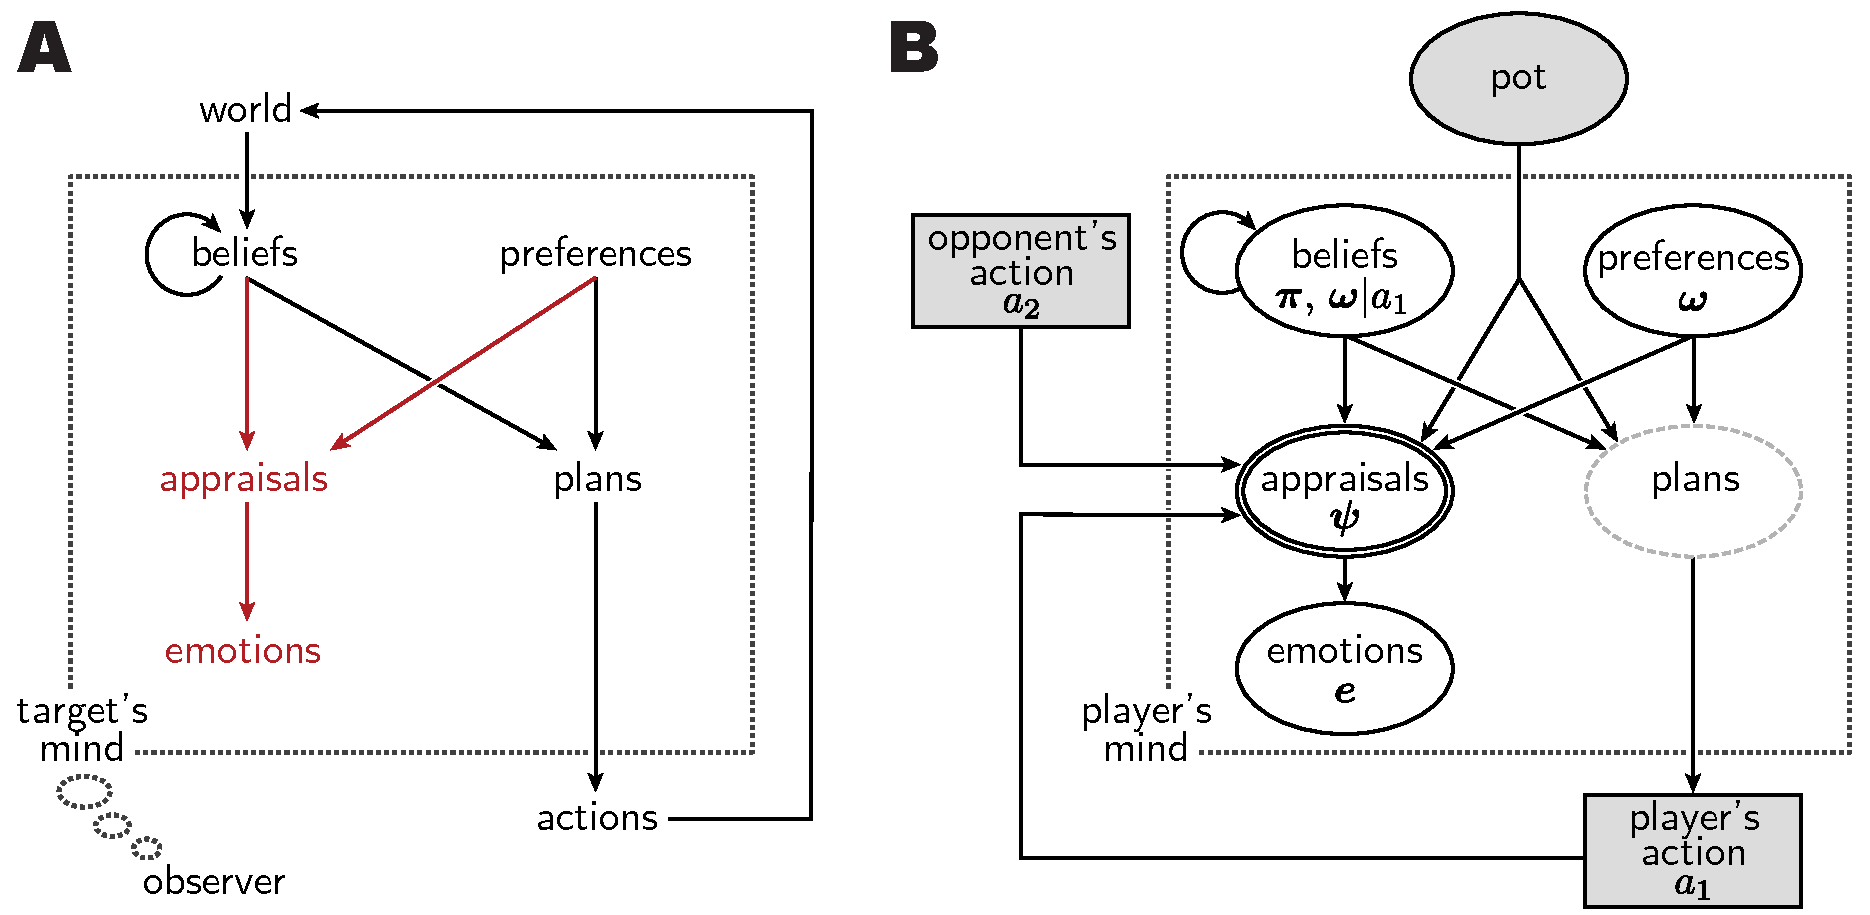
\includegraphics[width=1\textwidth,keepaspectratio]{figs/model_diagram.pdf}
	\caption{\textbf{Emotion prediction as inference over an intuitive Theory of Mind.} 
	Hypotheses about how human observers reason about others' emotions can be formalized as probabilistic generative models.
	}
	\label{fig:supp:dag}
\end{figure}

\subsection{Example Table}

\begin{table}[h!]
\begin{center} 
\caption{Sample table title.} 
\label{sample-table} 
\vskip 0.12in
\begin{tabular}{ll} 
\hline
Error type    &  Example \\
\hline
Take smaller        &   63 - 44 = 21 \\
Always borrow~~~~   &   96 - 42 = 34 \\
0 - N = N           &   70 - 47 = 37 \\
0 - N = 0           &   70 - 47 = 30 \\
\hline
\end{tabular} 
\end{center} 
\end{table}



\end{document}
